\section{Especificação dos tokens}
Os analisadores léxico e sintático serão implementados na linguagem C++.
A máquina de estados do analisador léxico (único implementado no momento) foi feita utilizando a ferramenta
\textit{Finite State Machine Designer} (https://www.cs.unc.edu/~otternes/comp455/fsm\textunderscore designer/) e
através de um \textit{script} \textit{Python} um arquivo contendo a tabela de transições é gerado e utilizado no
programa principal.
A tabela \ref{tab:tokens} mostra os nomes simbólicos dos \textit{tokens} acompanhados de seus valores numéricos.
A figura \ref{fig:maquina_estados} mostra a máquina de estados construída.
A ferramenta possibilita a exportação no formato \textit{json}, que é utilizado para a geração dos arquivos.
\begin{center}

    \begin{longtable}[c]{ | l | r | }
        \label{tab:tokens}
        \caption{Enumeração das categorias dos \textit{tokens}.}
        \endfirsthead
        \endhead
        \endfoot
        \endlastfoot
        \hline
        Nome simbólico & Valor numérico \\
        \hline
        Assignment & 0 \\
Bool & 1 \\
Break & 2 \\
Character & 3 \\
CloseBraces & 4 \\
CloseBrackets & 5 \\
CloseParenthesis & 6 \\
Comma & 7 \\
Dot & 8 \\
Ellipsis & 9 \\
Else & 10 \\
EndOfLine & 11 \\
Float & 12 \\
For & 13 \\
Identifier & 14 \\
If & 15 \\
In & 16 \\
Integer & 17 \\
OpAdd & 18 \\
OpAnd & 19 \\
OpDiv & 20 \\
OpEq & 21 \\
OpGt & 22 \\
OpGte & 23 \\
OpLt & 24 \\
OpLte & 25 \\
OpMod & 26 \\
OpMul & 27 \\
OpNeq & 28 \\
OpNot & 29 \\
OpOr & 30 \\
OpSub & 31 \\
OpenBraces & 32 \\
OpenBrackets & 33 \\
OpenParenthesis & 34 \\
Print & 35 \\
Return & 36 \\
Scan & 37 \\
SemiColon & 38 \\
Skip & 39 \\
String & 40 \\
TypeBool & 41 \\
TypeChar & 42 \\
TypeFloat & 43 \\
TypeInt & 44 \\
TypeString & 45 \\
Void & 46 \\
While & 47 \\
        \hline
    \end{longtable}
\end{center}

\begin{figure}
    \centering
    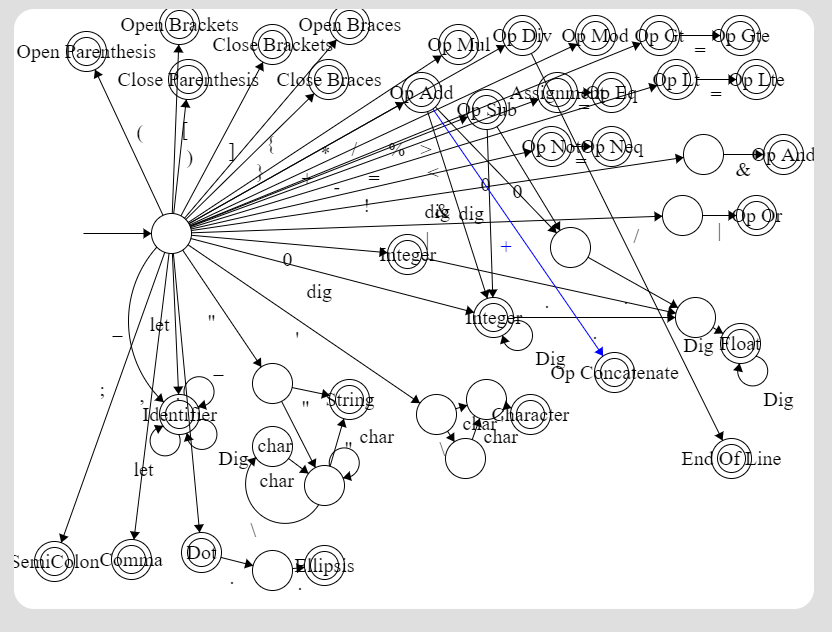
\includegraphics[width=\textwidth, caption=]{imagens/state_machine}
    \caption{Máquina de estados do autômato}
    \label{fig:maquina_estados}
\end{figure}

\begin{table}[!h]
    \centering
    \begin{tabular}{ | c | c |}
        \hline
        Padrão & Expressão regular                         \\
        \hline
        dig    & \texttt{'[1-9]'}                          \\
        Dig    & \texttt{'[0-9]'}                          \\
        let    & \texttt{'[a-zA-Z]'}                       \\
        char   & \texttt{[\textbackslash n-\textasciitilde]} \\
        \hline
    \end{tabular}
    \caption{Expressões regulares auxiliares}
    \label{tab:expressoes-auxiliares}
\end{table}


\begin{center}
    \centering
    \begin{longtable}[c]{ | l | c | }
        \label{tab:expressoes-regulares}
        \caption{Expressões regulares das categorias dos \textit{tokens}.}
        \endfirsthead
        \endhead
        \endfoot
        \endlastfoot
        \hline
        Categoria & Expressão regular\\
        \hline
        Arrow & \texttt{->}\\
Assignment & \texttt{=}\\
Bool & \texttt{true|false}\\
Break & \texttt{break}\\
Character & \texttt{'\{char\}'}\\
CloseBraces & \texttt{\}}\\
CloseBrackets & \texttt{]}\\
CloseParentheses & \texttt{)}\\
Comma & \texttt{,}\\
Dot & \texttt{.}\\
Ellipsis & \texttt{...}\\
Else & \texttt{else}\\
EndOfLine & \texttt{//}\\
Float & \texttt{[+-]?\{Dig\}+.\{Dig\}+}\\
For & \texttt{for}\\
Func & \texttt{func}\\
Identifier & \texttt{[\_\{let\}][\{let\}\{Dig\}\_]*}\\
If & \texttt{if}\\
In & \texttt{in}\\
Integer & \texttt{[+-]?0|(\{dig\}\{Dig\}*)}\\
OpAdd & \texttt{+}\\
OpAnd & \texttt{\&\&}\\
OpConcatenate & \texttt{++}\\
OpDiv & \texttt{/}\\
OpEq & \texttt{==}\\
OpGt & \texttt{>}\\
OpGte & \texttt{>=}\\
OpLt & \texttt{<}\\
OpLte & \texttt{<=}\\
OpMod & \texttt{\%}\\
OpMul & \texttt{*}\\
OpNeq & \texttt{!=}\\
OpNot & \texttt{!}\\
OpOr & \texttt{||}\\
OpSub & \texttt{-}\\
OpenBraces & \texttt{\{}\\
OpenBrackets & \texttt{[}\\
OpenParentheses & \texttt{(}\\
Print & \texttt{print}\\
Return & \texttt{return}\\
Scan & \texttt{scan}\\
SemiColon & \texttt{;}\\
Skip & \texttt{skip}\\
String & \texttt{\textbackslash"(\{char\}|(\textbackslash\textbackslash\{char\}))*\textbackslash"}\\
TypeBool & \texttt{bool}\\
TypeChar & \texttt{char}\\
TypeFloat & \texttt{float}\\
TypeInt & \texttt{int}\\
TypeString & \texttt{string}\\
Void & \texttt{void}\\
While & \texttt{while}
        \hline
    \end{longtable}
\end{center}